% !TeX program = xelatex
\documentclass[a4paper,10pt]{article}

% ============================================================================
% សន្លឹកកិច្ចការសិស្សបំពេញចន្លោះ ស-ខ្មៅ និងប្លង់ក្ដារខៀន/ចម្លើយគ្រូ (គ្មាន LCD / គ្មានកន្ត្រៃ)
% មេរៀនទី៣ (២.៣–២.៤)៖ ការបញ្ចុះតម្លៃ និងបម្រែបម្រួលភាគរយ — ត្រូវគ្នា ១០០% នឹង LS_Plan_PCT323.tex
% ============================================================================
\usepackage[a4paper, left=1.0cm, right=1.0cm, top=0.75cm, bottom=1.00cm, footskip=0.52cm]{geometry}
\usepackage{amsmath}
\usepackage{unicode-math}
\usepackage{fontspec}
\usepackage{array, colortbl}
\usepackage[table]{xcolor}
\usepackage{enumitem}
\usepackage{pifont}
\usepackage{fancyhdr}
\usepackage{lastpage}
\usepackage{tikz}
\usepackage[most]{tcolorbox}
\usetikzlibrary{calc, arrows.meta, decorations.pathreplacing, positioning, babel}

\makeatletter
\let\@expl@@@mark@update@singlecol@structures@@\relax
\makeatother

\providecommand{\NGSFindFonts}{%
  \IfFileExists{C:/Windows/Fonts/cambria.ttc}{%
    \def\NGSSysPath{C:/Windows/Fonts/}%
    \def\NGSUserPath{C:/Users/KIT/AppData/Local/Microsoft/Windows/Fonts/}%
  }{%
    \IfFileExists{./fonts/KhmerOSsiemreap.ttf}{\def\NGSSysPath{./fonts/}\def\NGSUserPath{./fonts/}}{%
    \IfFileExists{../fonts/KhmerOSsiemreap.ttf}{\def\NGSSysPath{../fonts/}\def\NGSUserPath{../fonts/}}{%
    \IfFileExists{../../fonts/KhmerOSsiemreap.ttf}{\def\NGSSysPath{../../fonts/}\def\NGSUserPath{../../fonts/}}{%
    \IfFileExists{../../../fonts/KhmerOSsiemreap.ttf}{\def\NGSSysPath{../../../fonts/}\def\NGSUserPath{../../../fonts/}}{%
    \IfFileExists{../../../../fonts/KhmerOSsiemreap.ttf}{\def\NGSSysPath{../../../../fonts/}\def\NGSUserPath{../../../../fonts/}}{%
    \IfFileExists{../../../../../fonts/KhmerOSsiemreap.ttf}{\def\NGSSysPath{../../../../../fonts/}\def\NGSUserPath{../../../../../fonts/}}{%
    \IfFileExists{../../../../../../fonts/KhmerOSsiemreap.ttf}{\def\NGSSysPath{../../../../../../fonts/}\def\NGSUserPath{../../../../../../fonts/}}{%
      \def\NGSSysPath{../../../../../../../fonts/}\def\NGSSysPath{../../../../../../../fonts/}%
    }}}}}}}%
  }%
}
\NGSFindFonts

\setmathfont[Path={\NGSSysPath}, FontIndex=1, Scale=1.02]{cambria.ttc}
\defaultfontfeatures{Ligatures=TeX}

\setmainfont[
  Path={\NGSUserPath}, Extension=.ttf, Script=Khmer,
  BoldFont={KhmerOSsiemreap}, BoldFeatures={FakeBold=1.8},
  ItalicFont={KhmerOSsiemreap}, ItalicFeatures={FakeSlant=0.25},
  BoldItalicFont={KhmerOSsiemreap}, BoldItalicFeatures={FakeBold=1.8, FakeSlant=0.25}
]{KhmerOSsiemreap}

\newfontfamily\muol[Path={\NGSUserPath}, Extension=.ttf, Script=Khmer]{KhmerOSmuollight}
\newfontfamily\TimesEn[Path={\NGSSysPath}, Extension=.ttf, BoldFont={timesbd}, ItalicFont={timesi}, BoldItalicFont={timesbi}]{times}
\newfontfamily\CalibriFont[Path={\NGSSysPath}, Extension=.ttf]{calibri}

\XeTeXlinebreaklocale "km"
\XeTeXlinebreakskip = 0pt plus 1pt minus 0.1pt

\definecolor{panelgray}{gray}{0.94}
\definecolor{headgray}{gray}{0.85}
\definecolor{midgray}{gray}{0.76}

\pagestyle{fancy}
\fancyhf{}
\renewcommand{\headrulewidth}{0pt}
\fancyfoot[L]{\fontsize{7.4pt}{9.5pt}\selectfont អនុវិទ្យាល័យព្រះក្រសាំង \en{|} គ្រូ៖ ហុក ប៊ុនថែន \en{|} មេរៀនទី៣ (២\en{.}៣--២\en{.}៤) ការបញ្ចុះតម្លៃ និងបម្រែបម្រួលភាគរយ \en{|} ថ្ងៃចន្ទ ទី២៣ ខែវិច្ឆិកា ឆ្នាំ២០២៦}
\fancyfoot[R]{\fontsize{7.8pt}{9.5pt}\selectfont ទំព័រ \en{\thepage\ / \pageref{LastPage}}}

\setlength{\parindent}{0pt}
\setlength{\parskip}{0pt}
\setlength{\tabcolsep}{4pt}

\newcommand{\en}[1]{{\TimesEn #1}}
\newcommand{\enbf}[1]{{\TimesEn\bfseries #1}}
\newcommand{\unit}[1]{\,\text{\en{#1}}}
\newcommand{\riel}{\,\text{៛}}
\newcommand{\usd}{\,\text{\en{\$}}}
\newcommand{\cnum}[1]{\mbox{\fontsize{10pt}{12pt}\selectfont\ding{\numexpr181+#1\relax}}}
\newcommand{\chkbox}{\tikz[baseline=-0.15ex]\draw[black, line width=0.85pt, fill=white] (0,0) rectangle (0.24cm,0.24cm);}
\newcommand{\ansbox}[1][1.35cm]{\,\tikz[baseline=-0.65ex]\draw[black, line width=0.65pt, fill=white] (0,0) rectangle (#1, 0.42cm);\,}
\newcommand{\dotline}[1][2.2cm]{\makebox[#1]{\dotfill}}

\newcommand{\pagebanner}[2]{%
  \begin{tcolorbox}[
    enhanced, sharp corners, colback=headgray, colframe=black,
    boxrule=1.05pt, boxsep=1pt, top=2.5pt, bottom=2.5pt, left=6pt, right=6pt,
    after skip=3.5pt
  ]
    {\muol\fontsize{9.0pt}{13.2pt}\selectfont #1}\hfill{\fontsize{8.0pt}{11.2pt}\selectfont\textbf{#2}}
  \end{tcolorbox}%
}

\newcommand{\secstrip}[2]{%
  \vspace{3pt}%
  \begin{tcolorbox}[
    enhanced, sharp corners, colback=panelgray, colframe=black,
    boxrule=0.8pt, boxsep=0.8pt, top=2pt, bottom=2pt, left=5pt, right=5pt,
    after skip=3pt
  ]
    {\muol\fontsize{8.5pt}{12.2pt}\selectfont #1}\hfill{\fontsize{7.8pt}{10.8pt}\selectfont\textit{#2}}
  \end{tcolorbox}%
}

\newcolumntype{L}[1]{>{\raggedright\arraybackslash}p{#1}}
\newcolumntype{C}[1]{>{\centering\arraybackslash}p{#1}}

\begin{document}
\fontsize{9.5pt}{14.5pt}\selectfont

% ============================================================================
% ទំព័រទី ១៖ សន្លឹកកិច្ចការសិស្ស (ផ្នែកមុខ៖ E1 -> E2 -> E3)
% ============================================================================
\pagebanner{សន្លឹកកិច្ចការសិស្ស \enbf{(}២\enbf{.}៣\enbf{--}២\enbf{.}៤ ការបញ្ចុះតម្លៃ និងបម្រែបម្រួលភាគរយ\enbf{)} \enbf{--} ផ្នែកមុខ}{ថ្នាក់ទី៨ \en{|} សៀវភៅគោល ទំ.៣៣--៣៤}

\begin{tcolorbox}[
  enhanced, sharp corners, colback=white, colframe=black,
  boxrule=0.8pt, boxsep=1.5pt, top=3.5pt, bottom=3.5pt, left=5pt, right=5pt,
  after skip=4pt
]
  \fontsize{9.0pt}{13.0pt}\selectfont
  \textbf{ឈ្មោះសិស្ស៖} \dotline[4.3cm] \quad
  \textbf{សមាជិកក្រុម៖} \dotline[4.3cm] \quad
  \textbf{ថ្នាក់ទី៖} ៨\dotline[0.9cm] \quad
  \textbf{ក្រុមទី៖} \dotline[1.0cm]
\end{tcolorbox}

% --- E1 Engage ---
\secstrip{ផ្នែកទី ១ \enbf{(E1 - Engage)} ៖ បេសកកម្មស្លាកបញ្ចុះតម្លៃនៅហាងសម្លៀកបំពាក់}{រយៈពេល ៣ នាទី (គូស \ding{51} ក្នុង \chkbox)}

\begin{tcolorbox}[
  enhanced, sharp corners, colback=white, colframe=black,
  boxrule=0.8pt, boxsep=1.5pt, top=3.5pt, bottom=3.5pt, left=5pt, right=5pt
]
  ហាងលក់សម្លៀកបំពាក់មួយដំឡើងថ្លៃអាវពី \textbf{$100\,000\riel$} ឡើង \textbf{$20\%$} បានថ្លៃថ្មី \textbf{$120\,000\riel$} ។ មួយសប្ដាហ៍ក្រោយមក ហាងប្រកាស\textbf{បញ្ចុះតម្លៃ $20\%$} លើថ្លៃថ្មីនោះ!\\[2.5pt]
  $\bullet$ \textbf{ការទស្សន៍ទាយរបស់ក្រុមអ្នក៖}\quad
  \chkbox\ ត្រឡប់មក \textbf{$100\,000\riel$} ដដែល \qquad
  \chkbox\ នៅសល់តែ \textbf{$96\,000\riel$} (ទាបជាងដើម!)\\[2pt]
  $\bullet$ \textbf{ហេតុផលខ្លី៖} ការបញ្ចុះតម្លៃ $20\%$ លើកទី ២ គឺគណនាលើតម្លៃគោល \dotline[3.0cm] $\riel$ ។
\end{tcolorbox}

\vfill

% --- E2 Explore ---
\secstrip{ផ្នែកទី ២ \enbf{(E2 - Explore)} ៖ ការបញ្ចុះតម្លៃ និងមេគុណបម្រែបម្រួលភាគរយ}{រយៈពេល ១១ នាទី}

\textbf{សកម្មភាព ១ (\en{E2-A} — ៥ នាទី)៖ ការបញ្ចុះតម្លៃកាបូបដៃ និងសម្លៀកបំពាក់ (សៀវភៅគោល ទំ.៣៣--៣៤)}\\[2pt]
\begin{tcolorbox}[
  enhanced, sharp corners, colback=white, colframe=black,
  boxrule=0.8pt, boxsep=1.5pt, top=3.5pt, bottom=3.5pt, left=5pt, right=5pt
]
  តម្លៃលក់ខាងដើមនៃកាបូបដៃមួយគឺ $32\,000\riel$ និងសម្លៀកបំពាក់មួយកំផ្លេគឺ $36\,000\riel$ ។ នៅដំណាច់ឆ្នាំ គេលក់កាបូបដៃថ្លៃតែ $25\,600\riel$ និងលក់សម្លៀកបំពាក់បញ្ចុះថ្លៃ $30\%$ ៖\\[2.5pt]
  $\bullet$ \textbf{ក. កាបូបដៃ៖} ការបញ្ចុះតម្លៃ $= 32\,000 - 25\,600 =$ \dotline[1.7cm] $\riel \implies$ ភាគរយបញ្ចុះ $= \dfrac{\dots\dots\dots}{32\,000}\times 100\% =$ \ansbox[1.3cm] $\%$\\[2.5pt]
  $\bullet$ \textbf{ខ. សម្លៀកបំពាក់៖} ការបញ្ចុះថ្លៃ $30\%$ នៃ $36\,000\riel = \dfrac{30}{100}\times 36\,000 =$ \dotline[1.8cm] $\riel \implies$ ថ្លៃលក់ $=$ \ansbox[2.0cm] $\riel$
\end{tcolorbox}

\vspace{4pt}
\textbf{សកម្មភាព ២ (\en{E2-B} — ៦ នាទី)៖ មេគុណបម្រែបម្រួលភាគរយលើប្រាក់ខែកម្មករ $320\,000\riel$ (ទំ.៣៤)}\\[2pt]
\begin{tcolorbox}[
  enhanced, sharp corners, colback=white, colframe=black,
  boxrule=0.8pt, boxsep=1.5pt, top=3.5pt, bottom=3.5pt, left=5pt, right=5pt
]
  {\centering\renewcommand{\arraystretch}{1.28}
  \begin{tabular}{|L{4.8cm}|C{5.2cm}|L{7.0cm}|}
    \hline
    \cellcolor{headgray}\textbf{ករណីប្រែប្រួលប្រាក់ខែ} & \cellcolor{headgray}\textbf{ផលធៀប $\dfrac{\text{ប្រាក់ខែថ្មី}}{\text{ប្រាក់ខែដើម}}$} & \cellcolor{headgray}\textbf{ការគណនាប្រាក់ខែថ្មី (ដើម $= 320\,000\riel$)} \\ \hline
    \textbf{១) កើនឡើង $15\%$} ($100+15$) & $\dfrac{\text{ប្រាក់ខែថ្មី}}{\text{ប្រាក់ខែដើម}} = \dfrac{115}{100}$ & $\dfrac{115}{100}\times 320\,000 =$ \ansbox[2.2cm] $\riel$ \\ \hline
    \textbf{២) ថយចុះ $5\%$} ($100-5$) & $\dfrac{\text{ប្រាក់ខែថ្មី}}{\text{ប្រាក់ខែដើម}} = \dfrac{\dots\dots}{100}$ & $\dfrac{\dots\dots}{100}\times 320\,000 =$ \ansbox[2.2cm] $\riel$ \\ \hline
  \end{tabular}\par}
\end{tcolorbox}

\vfill

% --- E3 Explain ---
\secstrip{ផ្នែកទី ៣ \enbf{(E3 - Explain)} ៖ ដ្យាក្រាមព្រួញមេគុណទៅ–មក និងធនាគារហេតុផល \enbf{B\&W}}{រយៈពេល ៦ នាទី}

\begin{tcolorbox}[
  enhanced, sharp corners, colback=white, colframe=black,
  boxrule=0.95pt, boxsep=1.6pt, top=3.5pt, bottom=3.5pt, left=5.5pt, right=5.5pt
]
  $\bullet$ \textbf{រូបមន្ត ២.៣ (ទំ.៣៣)៖} ភាគរយការបញ្ចុះតម្លៃ $= \dfrac{\text{ការបញ្ចុះតម្លៃ}}{\dots\dots\dots\dots\dots\dots}\times 100\%$\\[3pt]
  $\bullet$ \textbf{រូបមន្ត ២.៤ (ទំ.៣៤--៣៥)៖} បម្រែបម្រួល $r\%$៖ \quad
  \textbf{ទៅមុខ៖} តម្លៃថ្មី $= \dfrac{100 \pm r}{100}\times$ តម្លៃដើម \quad\en{|}\quad
  \textbf{បញ្ច្រាស៖} តម្លៃដើម $= \dfrac{100}{\dots\dots\dots}\times$ តម្លៃថ្មី\\[3pt]
  \hrule height 0.5pt
  \vspace{2.5pt}
  {\fontsize{8.7pt}{12.5pt}\selectfont
  \textbf{ធនាគារហេតុផល (\en{Warrant Bank})៖}\quad
  \cnum{1} ថ្លៃលក់ខាងដើម $= 100\%$ ជានិច្ច \quad
  \cnum{2} \textbf{ព្រួញទៅមុខ} (ស្គាល់ដើម)៖ គុណនឹង $\frac{100\pm r}{100}$\\
  \cnum{3} \textbf{ព្រួញបញ្ច្រាស} (ស្គាល់ថ្មី រកដើម)៖ គុណនឹងប្រភាគចម្រាស $\frac{100}{100\pm r}$ \quad
  \cnum{4} ហាមយក $r\%$ នៃតម្លៃថ្មីទៅបូក/ដក!}
\end{tcolorbox}

\newpage

% ============================================================================
% ទំព័រទី ២៖ សន្លឹកកិច្ចការសិស្ស (ផ្នែកខាងខ្នង៖ E4 -> E5 -> កិច្ចការផ្ទះ)
% ============================================================================
\pagebanner{សន្លឹកកិច្ចការសិស្ស \enbf{(}២\enbf{.}៣\enbf{--}២\enbf{.}៤ ការបញ្ចុះតម្លៃ និងបម្រែបម្រួលភាគរយ\enbf{)} \enbf{--} ផ្នែកខាងខ្នង}{ថ្នាក់ទី៨ \en{|} សៀវភៅគោល ទំ.៣៤--៣៥, ៤២}

% --- E4 Elaborate ---
\secstrip{ផ្នែកទី ៤ \enbf{(E4 - Elaborate)} ៖ លំហាត់គំរូប្រាក់ខែដំឡើង \enbf{8\%} (ទៅមុខ ទល់នឹង បញ្ច្រាស ទំ.៣៤--៣៥)}{រយៈពេល ១០ នាទី}

\begin{tcolorbox}[
  enhanced, sharp corners, colback=white, colframe=black,
  boxrule=0.8pt, boxsep=1.8pt, top=3.5pt, bottom=3.5pt, left=5.5pt, right=5.5pt
]
  \textbf{លំហាត់គំរូ (ទំ.៣៤--៣៥)៖} កម្មករនៃក្រុមហ៊ុនអគ្គិសនីមួយត្រូវបានគេដំឡើងប្រាក់ខែប្រចាំខែចំនួន \textbf{$8\%$} ($100\% + 8\% =$ \dotline[1.3cm] $\%$) ៖\\[3pt]
  $\bullet$ \textbf{ក. លោកប៊ុនថា} ទទួលប្រាក់ខែដើម $540\,000\riel$ ក្នុង ១ ខែ ។ រកប្រាក់ខែថ្មីរបស់គាត់បន្ទាប់ពីដំឡើង $8\%$ (\cnum{2})៖\\
  \hspace*{0.35cm}$\text{ប្រាក់ខែថ្មី} = \dfrac{\dots\dots\dots}{100} \times 540\,000 =$ \ansbox[2.2cm] $\riel$\\[3pt]
  $\bullet$ \textbf{ខ. លោកស្រីចាន់ធី} ទទួលប្រាក់ខែថ្មី $518\,400\riel$ \textbf{បន្ទាប់ពីបានដំឡើងរួច} ។ រកប្រាក់ខែដើមរបស់គាត់ (\cnum{3})៖\\
  \hspace*{0.35cm}$\dfrac{\text{ប្រាក់ខែថ្មី}}{\text{ប្រាក់ខែដើម}} = \dfrac{108}{100} \implies \text{ប្រាក់ខែដើម} = \dfrac{100}{\dots\dots\dots} \times 518\,400 =$ \ansbox[2.2cm] $\riel$\\[3pt]
  {\fontsize{8.7pt}{12.2pt}\selectfont \textbf{ឆ្លុះបញ្ចាំង (\en{EIA Looking-Back} \cnum{4})៖} ហេតុអ្វីការគណនា $518\,400 - 8\%\times 518\,400 = 476\,928\riel$ ខុស? ព្រោះ $8\%$ គិតលើប្រាក់ខែ \dotline[2.0cm] មិនមែនលើប្រាក់ខែថ្មីទេ!}
\end{tcolorbox}

\vfill

% --- E5 Evaluate ---
\secstrip{ផ្នែកទី ៥ \enbf{(E5 - Evaluate)} ៖ លំហាត់ប្រតិបត្តិ សំណួរវិនិច្ឆ័យ \enbf{A--D} និងសំបុត្រចេញ}{រយៈពេល ១០ នាទី}

\noindent
\begin{minipage}[t]{9.25cm}
  \begin{tcolorbox}[
    enhanced, sharp corners, colback=white, colframe=black,
    boxrule=0.8pt, boxsep=1.5pt, top=3.5pt, bottom=3.5pt, left=4.5pt, right=4.5pt
  ]
    \textbf{១) ប្រតិបត្តិ (ទំ.៣៥ — កង់បញ្ចុះតម្លៃ $15\%$)៖}\\
    ទោចក្រយានមួយគ្រឿងបន្ទាប់ពីបញ្ចុះតម្លៃ $15\%$ នៅសល់តម្លៃត្រឹមតែ $846\,000\riel$ ។ រកតម្លៃដើម (\cnum{3})៖\\[2pt]
    $\bullet$ ភាគរយតម្លៃនៅសល់ $= 100\% - 15\% =$ \dotline[1.3cm] $\%$\\[2pt]
    $\bullet$ តម្លៃដើម $= \dfrac{100}{\dots\dots}\times 846\,000 \approx$ \ansbox[2.2cm] $\riel$
  \end{tcolorbox}
\end{minipage}%
\hfill
\begin{minipage}[t]{9.25cm}
  \begin{tcolorbox}[
    enhanced, sharp corners, colback=white, colframe=black,
    boxrule=0.8pt, boxsep=1.5pt, top=3.5pt, bottom=3.5pt, left=4.5pt, right=4.5pt
  ]
    \textbf{២) បិទបេសកកម្ម \en{E1} និងលំហាត់រហ័ស៖}\\
    $\bullet$ \textbf{បិទ \en{E1}៖} អាវថ្លៃថ្មី $120\,000\riel$ បញ្ចុះ $20\%$ លក់ថ្លៃ៖\\
    \hspace*{0.2cm}$\dfrac{80}{100}\times 120\,000 =$ \ansbox[2.0cm] $\riel$ ($\neq 100\,000\riel$!)\\[2pt]
    $\bullet$ កង្ហារមួយបញ្ចុះ $15\%$ នៅសល់ថ្លៃ $85\,000\riel$ ៖\\
    \hspace*{0.2cm}តម្លៃដើម $= \dfrac{100}{85}\times 85\,000 =$ \dotline[1.9cm] $\riel$
  \end{tcolorbox}
\end{minipage}

\vspace{4.5pt}
\begin{tcolorbox}[
  enhanced, sharp corners, colback=panelgray, colframe=black,
  boxrule=0.85pt, boxsep=1.6pt, top=3.5pt, bottom=3.5pt, left=5.5pt, right=5.5pt
]
  \textbf{៣) សំណួរវិនិច្ឆ័យ \en{A--D} (អាវមួយបញ្ចុះតម្លៃ $20\%$ នៅសល់ថ្លៃ $40\,000\riel$ តើថ្លៃដើមស្មើប៉ុន្មាន? លើកម្រាមដៃ ១--៤)៖}\\
  \textbf{\en{A.}} $48\,000\riel$ \qquad
  \textbf{\en{B.}} $32\,000\riel$ \qquad
  \textbf{\en{C.}} $\dfrac{100}{80}\times 40\,000 = 50\,000\riel$ \qquad
  \textbf{\en{D.}} $\dfrac{100}{120}\times 40\,000 \approx 33\,333\riel$\\[2.5pt]
  \hrule height 0.5pt
  \vspace{2.5pt}
  \textbf{៤) សំបុត្រចេញ ៦០ វិនាទី៖}
  (ក) សៀវភៅថ្លៃ $20\,000\riel$ បញ្ចុះ $15\%$ លក់ថ្លៃ \dotline[1.7cm] $\riel$ ។ \quad
  (ខ) ប្រាក់ខែឡើង $10\%$ បាន $330\,000\riel$ នោះប្រាក់ខែដើមគឺ \dotline[1.8cm] $\riel$ ។
\end{tcolorbox}

\vfill

\begin{tcolorbox}[
  enhanced, sharp corners, colback=white, colframe=black,
  boxrule=1.0pt, boxsep=1.6pt, top=3pt, bottom=3pt, left=5.5pt, right=5.5pt
]
  {\muol\fontsize{8.7pt}{12.2pt}\selectfont កិច្ចការផ្ទះ \enbf{(}សៀវភៅគោល ទំ\enbf{.}៣៤ ប្រតិបត្តិ និង ទំ\enbf{.}៤២ លេខ ១៤ ខ\enbf{)}}\\[2.5pt]
  \fontsize{8.6pt}{12.3pt}\selectfont
  $\bullet$ \textbf{ប្រតិបត្តិ (ទំ.៣៤)៖} មីងសារីទិញថាសចម្រៀង $300$ ថាស ក្នុង ១ ថាសថ្លៃ $3\,300\riel$ ។ ដំបូងគាត់លក់អស់ $200$ ថាស ក្នុង ១ ថាសថ្លៃ $3\,980\riel$ ហើយនៅសល់ពីនេះគាត់លក់បញ្ចុះតម្លៃ $15\%$ ។ ចូររកភាគរយប្រាក់ចំណេញរបស់គាត់ ។\\
  $\bullet$ \textbf{\#14 ខ (ទំ.៤២ — បន្តពី \#14 ក៖ មិនមែនប្រលោមលោក $3\,240$ ក្បាល, ប្រលោមលោក $1\,260$ ក្បាល)៖} បណ្ណាល័យបង្កើនសៀវភៅមិនមែនប្រលោមលោក $7\frac{1}{2}\%$ (ថ្លៃ $7\,500\riel$/ក្បាល) និងប្រលោមលោក $5\%$ (ថ្លៃ $2\,250\riel$/ក្បាល) ។ គណនា៖ \en{(i)} តម្លៃសរុបនៃសៀវភៅថ្មី និង \en{(ii)} ភាគរយកើនឡើងនៃសៀវភៅអានទាំងអស់ ។ \textbf{អានមុន៖} ២.៥ ការប្រាក់សាមញ្ញ (ទំ.៣៥--៣៧) ។
\end{tcolorbox}

\newpage

% ============================================================================
% ទំព័រទី ៣៖ ប្លង់ក្ដារខៀន (គ្មាន LCD) និងចម្លើយផ្ទៀងផ្ទាត់រហ័សសម្រាប់គ្រូ
% ============================================================================
\pagebanner{ទំព័រគ្រូបង្រៀន ៖ ប្លង់ក្ដារខៀន \enbf{(}គ្មាន \enbf{LCD)} និងចម្លើយផ្ទៀងផ្ទាត់រហ័ស}{២.៣--២.៤ ការបញ្ចុះតម្លៃ និងបម្រែបម្រួលភាគរយ \en{(PCT323)}}

\secstrip{១. គំរូប្លង់បែងចែកក្ដារខៀន ៣ ផ្នែក សម្រាប់ថ្នាក់រៀនគ្មាន \enbf{LCD}}{សម្រាប់គ្រូប្រើដីស/ហ្វឺត}

\begin{center}
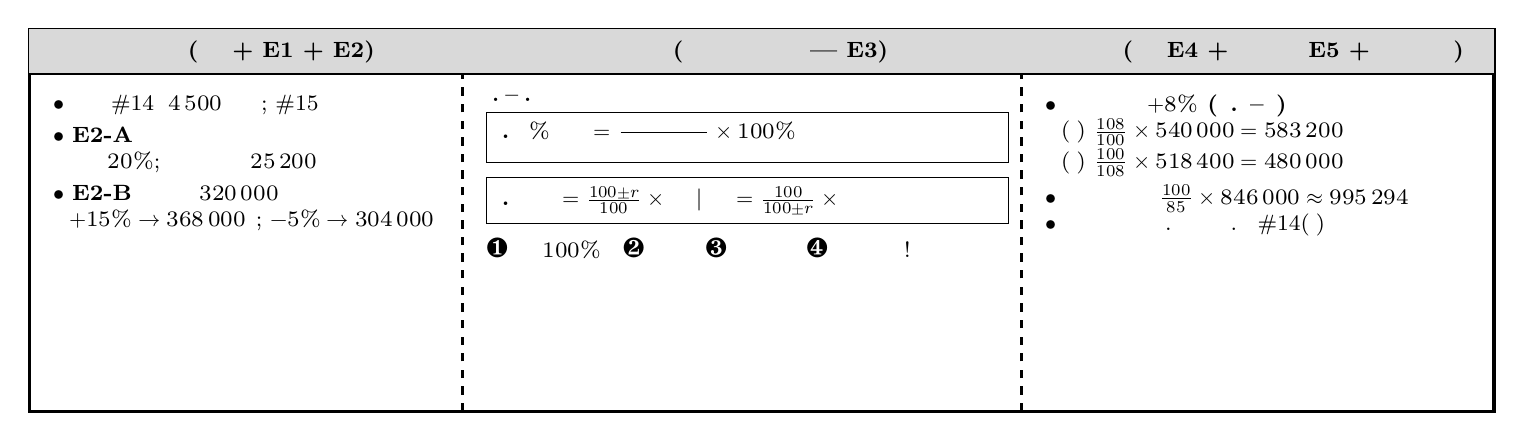
\begin{tikzpicture}[x=1cm, y=1cm, every node/.style={font=\footnotesize, text=black}]
  \draw[black, line width=1.2pt] (0,0) rectangle (18.6,4.85);
  \fill[headgray] (0,4.28) rectangle (18.6,4.85);
  \draw[black, line width=0.8pt] (0,4.28) -- (18.6,4.28);
  \draw[black, line width=0.85pt, dashed] (5.5,0) -- (5.5,4.28);
  \draw[black, line width=0.85pt, dashed] (12.6,0) -- (12.6,4.28);

  \node at (2.75,4.56) {\textbf{ផ្នែកឆ្វេង (កំណែ + \en{E1} + \en{E2})}};
  \node at (9.05,4.56) {\textbf{ផ្នែកកណ្ដាល (ខ្លឹមសារគោលរក្សាទុក — \en{E3})}};
  \node at (15.6,4.56) {\textbf{ផ្នែកស្ដាំ (គំរូ \en{E4} + ប្រតិបត្តិ \en{E5} + កិច្ចការផ្ទះ)}};

  \node[anchor=north west, align=left] at (0.18,4.14) {
    $\bullet$ \textbf{កំណែ៖} \#14ក $4\,500$ ក្បាល; \#15\\[2pt]
    $\bullet$ \textbf{\en{E2-A} បញ្ចុះតម្លៃ៖}\\
    \hspace*{0.2cm}កាបូប $20\%$; សម្លៀកបំពាក់ $25\,200\riel$\\[2pt]
    $\bullet$ \textbf{\en{E2-B} ប្រាក់ខែ $320\,000\riel$៖}\\
    \hspace*{0.2cm}$+15\% \to 368\,000\riel$; $-5\% \to 304\,000\riel$
  };

  \node[anchor=north west, align=left] at (5.68,4.14) {
    {\muol\fontsize{7.6pt}{11.5pt}\selectfont ២\enbf{.}៣\enbf{--}២\enbf{.}៤ ការបញ្ចុះតម្លៃ និងបម្រែបម្រួលភាគរយ}\\[3pt]
    \fbox{\parbox{6.4cm}{\textbf{២.៣៖} $\% \text{បញ្ចុះ} = \dfrac{\text{ការបញ្ចុះតម្លៃ}}{\text{ថ្លៃលក់ខាងដើម}}\times 100\%$}}\\[4pt]
    \fbox{\parbox{6.4cm}{\textbf{២.៤៖} ថ្មី $= \frac{100\pm r}{100}\times\text{ដើម}$ \en{|} ដើម $= \frac{100}{100\pm r}\times\text{ថ្មី}$}}\\[4pt]
    \cnum{1} ដើម $100\%$ \; \cnum{2} ទៅមុខ \; \cnum{3} បញ្ច្រាស \; \cnum{4} កុំដកពីថ្មី!
  };

  \node[anchor=north west, align=left] at (12.78,4.14) {
    $\bullet$ \textbf{គំរូប្រាក់ខែ $+8\%$ (ទំ.៣៤--៣៥)៖}\\
    \hspace*{0.2cm}(ក) $\frac{108}{100}\times 540\,000 = 583\,200\riel$\\
    \hspace*{0.2cm}(ខ) $\frac{100}{108}\times 518\,400 = 480\,000\riel$\\[2pt]
    $\bullet$ \textbf{ប្រតិបត្តិកង់៖} $\frac{100}{85}\times 846\,000 \approx 995\,294\riel$\\
    $\bullet$ \textbf{កិច្ចការផ្ទះ៖} ទំ.៣៤ និង ទំ.៤២ \#14(ខ)
  };
\end{tikzpicture}
\end{center}

\secstrip{២. ចម្លើយផ្ទៀងផ្ទាត់រហ័សសម្រាប់សន្លឹកកិច្ចការសិស្ស (ទំព័រ ១ និង ទំព័រ ២)}{\en{Answer Key}}

\begin{tcolorbox}[
  enhanced, sharp corners, colback=white, colframe=black,
  boxrule=0.8pt, boxsep=1.5pt, top=3pt, bottom=3pt, left=5pt, right=5pt,
  after skip=3.5pt
]
  \fontsize{8.8pt}{13.2pt}\selectfont
  $\bullet$ \textbf{ផ្នែក \en{E1}៖} នៅសល់តែ \textbf{$96\,000\riel$}; បញ្ចុះ $20\%$ លើកទី ២ គិតលើ \textbf{$120\,000\riel$} ។\\[2pt]
  $\bullet$ \textbf{ផ្នែក \en{E2}៖} \textbf{សកម្មភាព ១៖} (ក) បញ្ចុះ $6\,400\riel \implies \mathbf{20\%}$; (ខ) បញ្ចុះ $10\,800\riel \implies$ ថ្លៃលក់ $\mathbf{25\,200\riel}$ ។ \textbf{សកម្មភាព ២៖} កើន $15\% \to \mathbf{368\,000\riel}$; ថយ $5\%$ ($\frac{95}{100}$) $\to \mathbf{304\,000\riel}$ ។\\[2pt]
  $\bullet$ \textbf{ផ្នែក \en{E4}៖} មេគុណ $\mathbf{108\%}$; (ក) លោកប៊ុនថា $\mathbf{583\,200\riel}$; (ខ) លោកស្រីចាន់ធី $\frac{100}{108}\times 518\,400 = \mathbf{480\,000\riel}$ ($8\%$ គិតលើប្រាក់ខែ\textbf{ដើម}) ។\\[2pt]
  $\bullet$ \textbf{ផ្នែក \en{E5}៖} \textbf{១) កង់៖} នៅសល់ $85\% \implies \frac{100}{85}\times 846\,000 \approx \mathbf{995\,294.12\riel}$ ។ \textbf{២) បិទ \en{E1}៖} $\mathbf{96\,000\riel}$; កង្ហារ $\mathbf{100\,000\riel}$ ។ \textbf{៣) វិនិច្ឆ័យ \en{A--D}៖} ជម្រើស \textbf{\en{C}} ($50\,000\riel$) ។ \textbf{៤) សំបុត្រចេញ៖} (ក) $\mathbf{17\,000\riel}$; (ខ) $\mathbf{300\,000\riel}$ ។
\end{tcolorbox}

\secstrip{៣. ចម្លើយលម្អិតនៃកិច្ចការផ្ទះ (សម្រាប់ផ្ទៀងនៅដើមម៉ោងបន្ទាប់ ២.៥)}{សៀវភៅគោល ទំ.៣៤, ៤២}

\begin{tcolorbox}[
  enhanced, sharp corners, colback=white, colframe=black,
  boxrule=0.8pt, boxsep=1.5pt, top=3pt, bottom=3pt, left=5pt, right=5pt
]
  \fontsize{8.6pt}{12.8pt}\selectfont
  $\bullet$ \textbf{ប្រតិបត្តិ (ទំ.៣៤ — មីងសារីលក់ថាសចម្រៀង)៖} ថ្លៃដើមសរុប $= 300 \times 3\,300 = 990\,000\riel$ ។ លក់លើកទី ១ ($200$ ថាស) $= 200 \times 3\,980 = 796\,000\riel$ ។ ថាសនៅសល់ $100$ ថាសលក់បញ្ចុះ $15\%$ នៃ $3\,980\riel$ ($= 0.85 \times 3\,980 = 3\,383\riel$/ថាស) បានប្រាក់ $338\,300\riel$ ។ ប្រាក់លក់សរុប $= 796\,000 + 338\,300 = 1\,134\,300\riel \implies$ ប្រាក់ចំណេញ $= 144\,300\riel \implies$ ភាគរយប្រាក់ចំណេញ $= \dfrac{144\,300}{990\,000}\times 100\% = \dfrac{481}{33}\% \approx \mathbf{14.58\%}$ ។\\[3pt]
  $\bullet$ \textbf{\#14 ខ (ទំ.៤២)៖} សៀវភៅមិនមែនប្រលោមលោកកើន $\frac{7.5}{100}\times 3\,240 = 243$ ក្បាល (ថ្លៃ $243\times 7\,500 = 1\,822\,500\riel$) និងប្រលោមលោកកើន $\frac{5}{100}\times 1\,260 = 63$ ក្បាល (ថ្លៃ $63\times 2\,250 = 141\,750\riel$) ។ \en{(i)} តម្លៃសរុបនៃសៀវភៅថ្មី $= 1\,822\,500 + 141\,750 = \mathbf{1\,964\,250\riel}$ ។ \en{(ii)} ភាគរយកើនឡើងសរុប $= \dfrac{243 + 63}{4\,500}\times 100\% = \dfrac{306}{4\,500}\times 100\% = \mathbf{6.8\%}$ ។
\end{tcolorbox}

\end{document}
